\begin{figure}
    \centering
    \begin{tabular}[l]{ccc}
    \begin{subfigure}[c]{0.315\textwidth}
        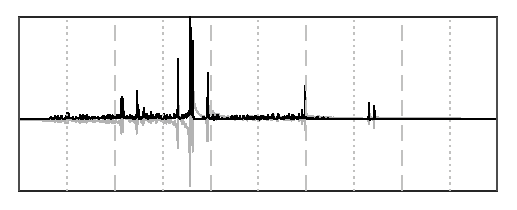
\includegraphics[width=0.95\textwidth,keepaspectratio]{images/PM_stages/pm_stages_1.eps}
        \caption{Original basis functions}
        \label{fig:PM_stages:basis functions}\vspace{0.2\baselineskip}
    \end{subfigure}&
    \begin{subfigure}[c]{0.315\textwidth}
        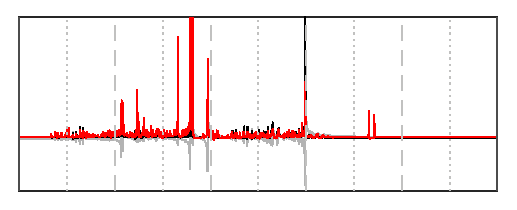
\includegraphics[width=0.95\textwidth,keepaspectratio]{images/PM_stages/pm_stages_2.eps}
        \caption{Modulated basis functions}
        \label{fig:PM_stages:modulated}\vspace{0.2\baselineskip}
    \end{subfigure}&
    \begin{subfigure}[c]{0.315\textwidth}
        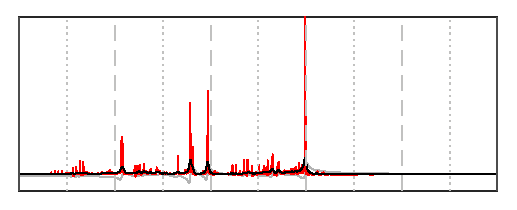
\includegraphics[width=0.95\textwidth,keepaspectratio]{images/PM_stages/pm_stages_3.eps}
        \caption{Voigt lineshape}
        \label{fig:PM_stages:B0 inhomogeneities}\vspace{0.2\baselineskip}
    \end{subfigure}\\[25pt]
    \begin{subfigure}[c]{0.315\textwidth}
        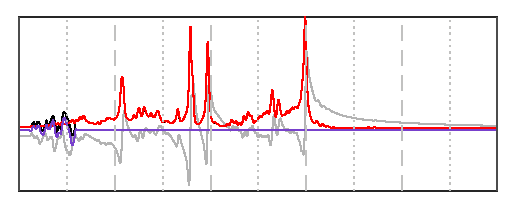
\includegraphics[width=0.95\textwidth,keepaspectratio]{images/PM_stages/pm_stages_4.eps}
        \caption{Residual Water}
        \label{fig:PM_stages:lineshape}\vspace{0.2\baselineskip}
    \end{subfigure}&
    \begin{subfigure}[c]{0.315\textwidth}
        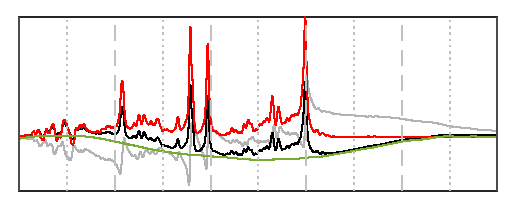
\includegraphics[width=0.95\textwidth,keepaspectratio]{images/PM_stages/pm_stages_5.eps}
        \caption{Baseline}
        \label{fig:PM_stages:phi1}\vspace{0.2\baselineskip}
    \end{subfigure}&
    \begin{subfigure}[c]{0.315\textwidth}
        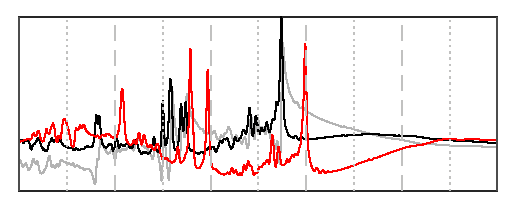
\includegraphics[width=0.95\textwidth,keepaspectratio]{images/PM_stages/pm_stages_6.eps}
        \caption{Frequency Shift}
        \label{fig:PM_stages:phi0}\vspace{0.2\baselineskip}\vspace{0.2\baselineskip}
    \end{subfigure}\\[25pt]
    \begin{subfigure}[c]{0.315\textwidth}
        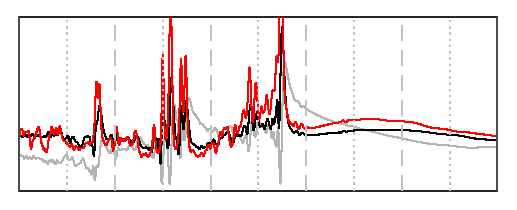
\includegraphics[width=0.95\textwidth,keepaspectratio]{images/PM_stages/pm_stages_7.eps}
        \caption{Eddy currents}
        \label{fig:PM_stages:fshift}\vspace{0.2\baselineskip}
    \end{subfigure}&
    \begin{subfigure}[c]{0.315\textwidth}
        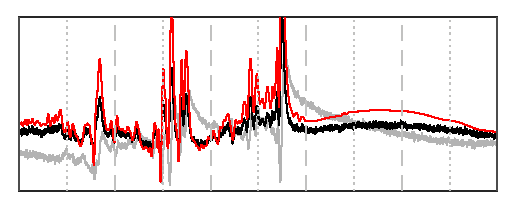
\includegraphics[width=0.95\textwidth,keepaspectratio]{images/PM_stages/pm_stages_8.eps}
        \caption{Noise}
        \label{fig:PM_stages:SNR}\vspace{0.2\baselineskip}
    \end{subfigure}&
    \begin{subfigure}[c]{0.315\textwidth}
        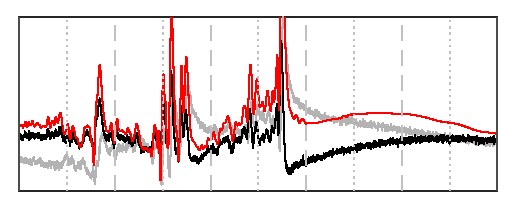
\includegraphics[width=0.95\textwidth,keepaspectratio]{images/PM_stages/pm_stages_9.eps}
        \caption{First-order phase}
        \label{fig:PM_stages:residual water}\vspace{0.2\baselineskip}
    \end{subfigure}\\[25pt]
    \begin{subfigure}[c]{0.315\textwidth}
        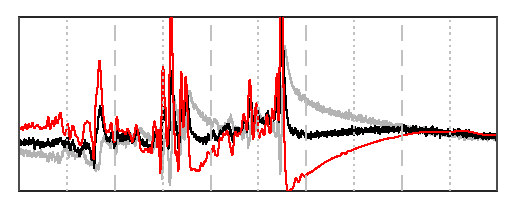
\includegraphics[width=0.95\textwidth,keepaspectratio]{images/PM_stages/pm_stages_10.eps}
        \vspace{0.5pt}
        \caption{Zero-order phase}
        \label{fig:PM_stages:baseline}
    \end{subfigure}&
    \begin{subfigure}[c]{0.315\textwidth}
        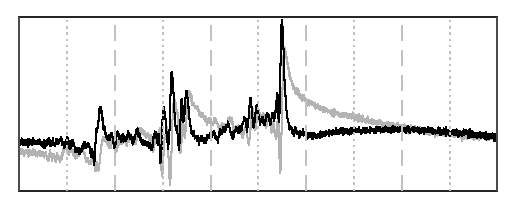
\includegraphics[width=0.95\textwidth,keepaspectratio]{images/PM_stages/pm_stages_11.eps}
        \vspace{0.5mm}
        \caption{Generated spectrum}
        \label{fig:PM_stages:generated spectrum}
    \end{subfigure}&
    \begin{subfigure}[c]{0.315\textwidth}
        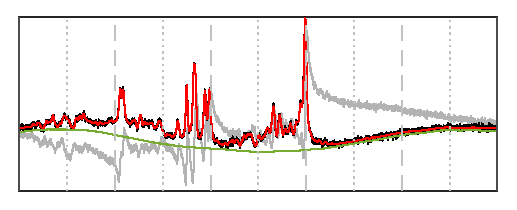
\includegraphics[width=0.95\textwidth,keepaspectratio]{images/PM_stages/pm_stages_12.eps} \smallskip
        \caption{Pre-processed spectrum}
        \label{fig:PM_stages:corrected}
    \end{subfigure}
    \end{tabular}
    \caption{This is a step-by-step progression through the physics model. The real and imaginary components are in black and grey, respectively. The red line includes only the metabolites and the offsets from the preceeding steps. \ref{fig:PM_stages:generated spectrum} is the final spectrum with all artifacts applied. \ref{fig:PM_stages:corrected} is the pre-processed spectrum with the phase and frequency shifts removed.}
    \label{fig:PM compilation}
\end{figure}
